\documentclass[aspectratio=43,11pt]{beamer}

\usepackage{fontspec}
\usepackage{graphicx}
\usepackage{tikz}
\usepackage{tabularx}
\usepackage{booktabs}
\usepackage{array}
\usetikzlibrary{positioning}

\newcommand{\UniversityName}{ĐẠI HỌC BÁCH KHOA HÀ NỘI}
\newcommand{\ReportType}{ĐỒ ÁN TỐT NGHIỆP}
\newcommand{\ReportTitle}{Xây dựng nền tảng Web UniTrack hỗ trợ giảng viên giám sát tiến độ dự án sinh viên}
\newcommand{\StudentName}{NGUYỄN LÊ TUẤN}
\newcommand{\StudentEmail}{student@example.com}
\newcommand{\MajorName}{Ngành Công nghệ thông tin}
\newcommand{\SupervisorName}{ThS. Tên Giảng Viên}
\newcommand{\FacultyName}{Khoa Công nghệ thông tin}
\newcommand{\SchoolName}{Trường Công nghệ thông tin và Truyền thông}
\newcommand{\ReportLocationDate}{HÀ NỘI, 06/2026}
\newcommand{\CommitmentDate}{Hà Nội, ngày 21 tháng 06 năm 2026}


\graphicspath{{hust-template-media/}{../assets/screenshots/}{../assets/diagrams/}}

\setsansfont{TeX Gyre Heros}
\setmainfont{TeX Gyre Heros}

\definecolor{hustred}{HTML}{B5121B}
\definecolor{hustdark}{HTML}{252525}
\definecolor{hustmuted}{HTML}{666666}
\definecolor{hustlight}{HTML}{F7F2F0}
\definecolor{hustline}{HTML}{D8C9C5}
\definecolor{unitblue}{HTML}{15365C}

\setbeamercolor{normal text}{fg=hustdark,bg=white}
\setbeamercolor{frametitle}{fg=hustdark,bg=white}
\setbeamercolor{structure}{fg=hustred}
\setbeamertemplate{navigation symbols}{}
\setbeamertemplate{itemize item}{\color{hustred}$\blacktriangleright$}
\setbeamertemplate{itemize subitem}{\color{hustred}$\bullet$}
\setbeamerfont{frametitle}{size=\Large,series=\bfseries}
\setbeamerfont{title}{size=\Large,series=\bfseries}

\newcommand{\deckfooter}{UniTrack | Đồ án tốt nghiệp}

\setbeamertemplate{frametitle}{%
  \vspace{0.15cm}%
  \begin{beamercolorbox}[wd=\paperwidth,ht=0.68cm,leftskip=0.55cm,rightskip=0.55cm]{frametitle}
    \insertframetitle
  \end{beamercolorbox}%
  \vspace{-0.18cm}%
  \begin{tikzpicture}[remember picture,overlay]
    \fill[hustred] (0.55,-0.08) rectangle (1.78,-0.13);
    \draw[hustline,line width=0.4pt] (1.86,-0.105) -- (11.8,-0.105);
  \end{tikzpicture}%
  \vspace{0.25cm}%
}

\setbeamertemplate{footline}{%
  \begin{tikzpicture}[remember picture,overlay]
    \draw[hustline,line width=0.35pt] (0.55,0.42) -- (11.72,0.42);
    \node[anchor=west,text=hustmuted,font=\scriptsize] at (0.55,0.18) {\deckfooter};
    \node[anchor=east,text=hustred,font=\scriptsize\bfseries] at (11.72,0.18) {\insertframenumber};
  \end{tikzpicture}%
  \vspace{0.52cm}%
}

\newcommand{\redtag}[1]{%
  \tikz[baseline=(x.base)]\node[fill=hustred,rounded corners=1.5pt,inner xsep=5pt,inner ysep=2pt,text=white,font=\scriptsize\bfseries] (x) {#1};%
}

\newcommand{\smallpath}[1]{{\scriptsize\texttt{#1}}}
\newcommand{\settemplatebg}[1]{%
  \usebackgroundtemplate{\includegraphics[width=\paperwidth,height=\paperheight]{#1}}%
}

\newenvironment{tightitems}{%
  \begin{itemize}\setlength\itemsep{0.28em}\setlength\parskip{0pt}\small
}{\end{itemize}}

\title{UniTrack}
\subtitle{Nền tảng Web hỗ trợ giảng viên giám sát tiến độ dự án sinh viên}
\author{\StudentName}
\institute{\SchoolName \\ \UniversityName}
\date{\ReportLocationDate}

\begin{document}

% 1
\settemplatebg{image3.png}
\begin{frame}[plain]
  \vspace{1.18cm}
  \centering
  
\includegraphics[height=0.6cm,keepaspectratio]{image13.png}\par
  \vspace{0.72cm}
  {\fontsize{27}{31}\selectfont\bfseries\color{hustred} UniTrack}\par
  \vspace{0.22cm}
  {\fontsize{15}{19}\selectfont\bfseries Xây dựng nền tảng Web hỗ trợ giảng viên giám sát tiến độ dự án sinh viên}\par
  \vspace{0.55cm}
  {\small Sinh viên: \textbf{\StudentName} \qquad GVHD: \textbf{\SupervisorName}}\par
  \vspace{0.15cm}
  {\small \SchoolName -- \UniversityName}\par
  \vspace{0.35cm}
  {\small \ReportLocationDate}
\end{frame}

% 2
\settemplatebg{image5.png}
\begin{frame}{Nội dung trình bày}
  \begin{columns}[T,totalwidth=\textwidth]
    \begin{column}{0.47\textwidth}
      \begin{enumerate}\small
        \item Bài toán và mục tiêu
        \item Phạm vi và quy trình nghiệp vụ
        \item Kiến trúc, công nghệ, dữ liệu
        \item Bảo mật, phân quyền, toàn vẹn
      \end{enumerate}
    \end{column}
    \begin{column}{0.47\textwidth}
      \begin{enumerate}\setcounter{enumi}{4}\small
        \item Giao diện và luồng sử dụng
        \item Dấu vết triển khai trong codebase
        \item Kiểm thử, kết quả, hạn chế
        \item Hướng phát triển
      \end{enumerate}
    \end{column}
  \end{columns}

  \vspace{0.55cm}
  \begin{block}{Thông điệp chính}
    \small UniTrack không chỉ quản lý danh sách công việc, mà chuẩn hóa workflow \textbf{Giảng viên -- Dự án -- Nhiệm vụ -- Bài nộp -- Duyệt bài} với quyền và dữ liệu được kiểm soát rõ ràng.
  \end{block}
\end{frame}

% 3
\settemplatebg{image6.png}
\begin{frame}{Bài toán đặt ra}
  \begin{columns}[T,totalwidth=\textwidth]
    \begin{column}{0.49\textwidth}
      \redtag{Hiện trạng}
      \begin{tightitems}
        \item Thông tin dự án nằm rải rác trong email, chat, bảng tính, thư mục file.
        \item Khó xác định nhiệm vụ nào quá hạn, bài nào đang chờ duyệt.
        \item File minh chứng dễ mất liên kết với quyết định đánh giá.
      \end{tightitems}
    \end{column}
    \begin{column}{0.49\textwidth}
      \redtag{Nhu cầu}
      \begin{tightitems}
        \item Giảng viên cần hàng đợi ưu tiên và lịch sử phản hồi.
        \item Sinh viên cần nơi xem nhiệm vụ, nộp tiến độ, đọc phản hồi.
        \item Quản trị viên cần kiểm soát tài khoản, vai trò, trạng thái.
      \end{tightitems}
    \end{column}
  \end{columns}

  \vspace{0.5cm}
  \centering
  \colorbox{hustlight}{\parbox{0.9\textwidth}{\centering\small Cần một hệ thống lấy \textbf{dự án} làm trục dữ liệu, không phụ thuộc ghi nhớ thủ công.}}
\end{frame}

% 4
\settemplatebg{image7.png}
\begin{frame}{Mục tiêu và phạm vi}
  \begin{columns}[T,totalwidth=\textwidth]
    \begin{column}{0.52\textwidth}
      \redtag{Mục tiêu}
      \begin{tightitems}
        \item Xây dựng Web platform giám sát dự án sinh viên.
        \item Dashboard theo vai trò: quản trị viên, giảng viên, sinh viên.
        \item Quản lý Workspace, dự án, nhóm, mốc, nhiệm vụ.
        \item Hỗ trợ nộp bài, duyệt bài, tài nguyên và minh chứng.
      \end{tightitems}
    \end{column}
    \begin{column}{0.42\textwidth}
      \redtag{Giữ phạm vi gọn}
      \begin{tightitems}
        \item Không đăng ký công khai.
        \item Không chat/mạng xã hội.
        \item Không chấm điểm số/rubric phức tạp.
        \item Tập trung workflow lõi của dự án.
      \end{tightitems}
    \end{column}
  \end{columns}
\end{frame}

% 5
\settemplatebg{image8.png}
\begin{frame}{Quy trình nghiệp vụ chính}
  \centering
  \begin{tikzpicture}[node distance=0.23cm, every node/.style={font=\scriptsize}]
    \tikzset{flowstep/.style={draw=hustred,thick,rounded corners,align=center,minimum width=1.72cm,minimum height=0.78cm,fill=white}}
    \node[flowstep] (a) {Admin\\tạo tài khoản};
    \node[flowstep,right=of a] (b) {Giảng viên\\tạo dự án};
    \node[flowstep,right=of b] (c) {Kế hoạch\\nhiệm vụ};
    \node[flowstep,right=of c] (d) {Sinh viên\\nộp bài};
    \node[flowstep,right=of d] (e) {Giảng viên\\duyệt bài};
    \draw[->,hustred,thick] (a) -- (b);
    \draw[->,hustred,thick] (b) -- (c);
    \draw[->,hustred,thick] (c) -- (d);
    \draw[->,hustred,thick] (d) -- (e);
  \end{tikzpicture}

  \vspace{0.55cm}
  \begin{columns}[T,totalwidth=\textwidth]
    \begin{column}{0.48\textwidth}
      \redtag{Luật nghiệp vụ}
      \begin{tightitems}
        \item Chỉ sinh viên active trong dự án mới được giao việc.
        \item Một nhiệm vụ chỉ có một bài đang chờ duyệt.
        \item Dự án active/on-hold/completed/archived quyết định thao tác ghi.
      \end{tightitems}
    \end{column}
    \begin{column}{0.48\textwidth}
      \redtag{Tác nhân}
      \begin{tightitems}
        \item Quản trị viên: tài khoản, dashboard toàn cục.
        \item Giảng viên: dự án, nhóm, nhiệm vụ, review.
        \item Sinh viên: xem việc, nộp bài, theo dõi phản hồi.
      \end{tightitems}
    \end{column}
  \end{columns}
\end{frame}

% 6
\settemplatebg{image9.png}
\begin{frame}{Kiến trúc tổng quan}
  \begin{columns}[T,totalwidth=\textwidth]
    \begin{column}{0.45\textwidth}
      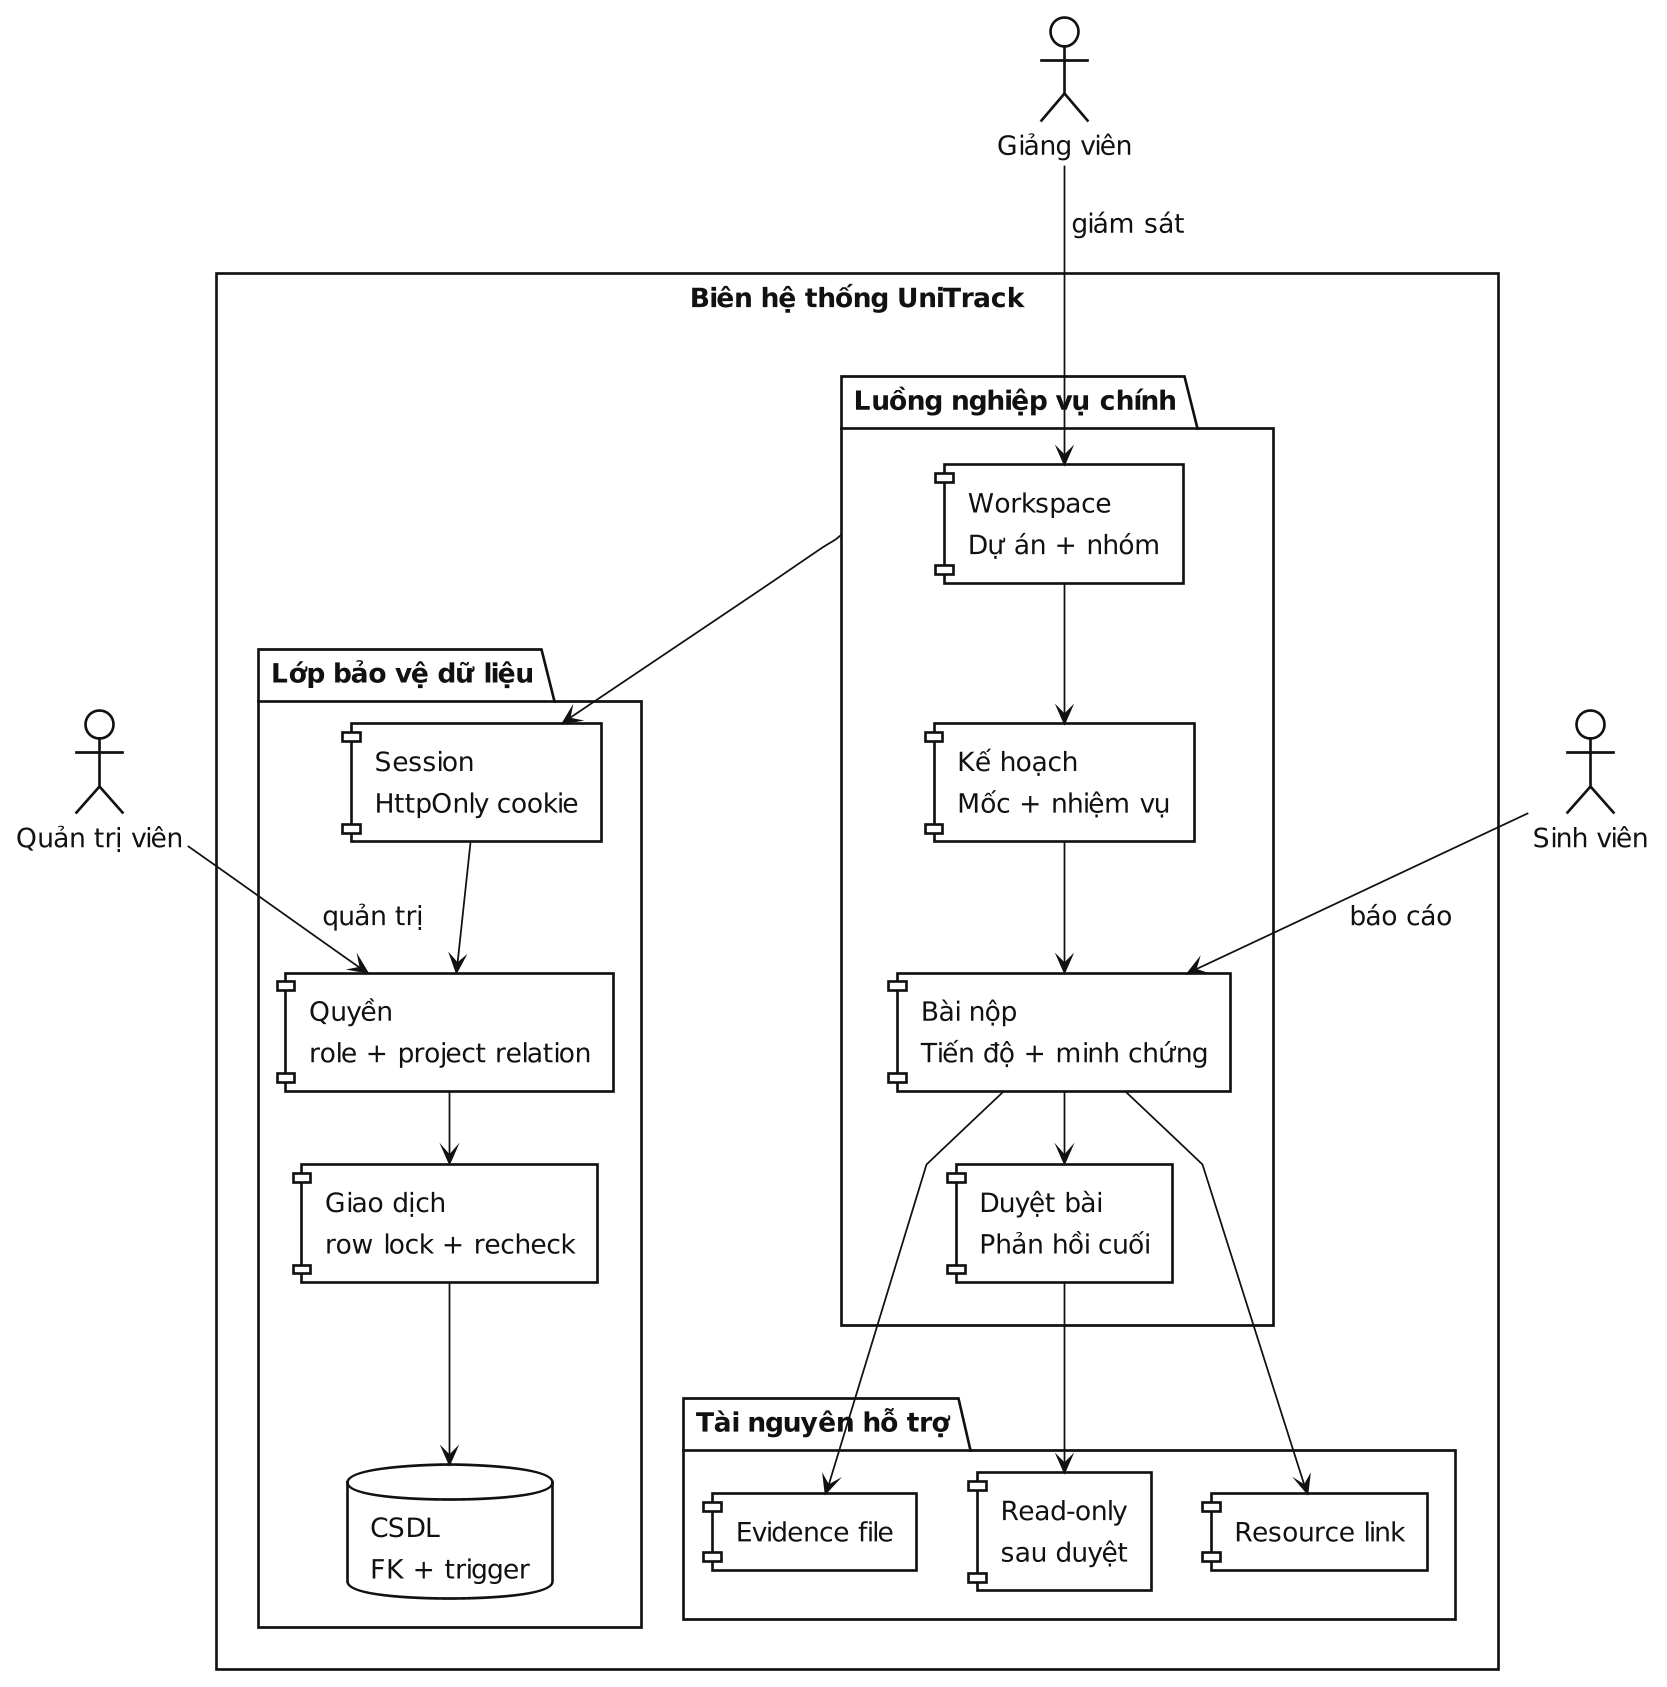
\includegraphics[width=\linewidth,height=0.72\textheight,keepaspectratio]{solution-overview.png}
    \end{column}
    \begin{column}{0.51\textwidth}
      \begin{tightitems}
        \item \textbf{Frontend}: React SPA, route guard, query cache.
        \item \textbf{Backend}: Go REST API dưới \texttt{/api/v1}.
        \item \textbf{Database}: PostgreSQL, migration, ràng buộc dữ liệu.
        \item \textbf{Storage}: local dev, Cloudflare R2 private production.
      \end{tightitems}
      \vspace{0.25cm}
      \colorbox{hustlight}{\parbox{0.95\linewidth}{\small Giao diện hướng dẫn thao tác; backend quyết định quyền; database bảo vệ invariant.}}
    \end{column}
  \end{columns}
\end{frame}

% 7
\settemplatebg{image10.png}
\begin{frame}{Công nghệ sử dụng}
  \renewcommand{\arraystretch}{1.22}
  \small
  \begin{tabularx}{\textwidth}{>{\bfseries\color{hustred}}p{2.6cm}X}
    Frontend & React, TypeScript, Vite, Tailwind CSS, shadcn/Radix, TanStack Query, Zustand \\
    Backend & Go, chi, pgx, REST API, raw SQL, strict JSON decoder \\
    Database & PostgreSQL, goose migrations, khóa ngoại, unique index, trigger deferred \\
    Storage & Local filesystem khi phát triển, Cloudflare R2 private khi production \\
    Kiểm thử & Go test, Playwright, migration validation, lint/build frontend \\
    Triển khai & Vercel, Render, Neon, Cloudflare R2
  \end{tabularx}

  \vspace{0.35cm}
  \begin{block}{Lý do chọn}
    \small Stack gọn, dễ triển khai, đủ mạnh cho bài toán nhiều trạng thái, nhiều quyền và ràng buộc dữ liệu quan hệ.
  \end{block}
\end{frame}

% 8
\settemplatebg{image11.png}
\begin{frame}{Thiết kế dữ liệu}
  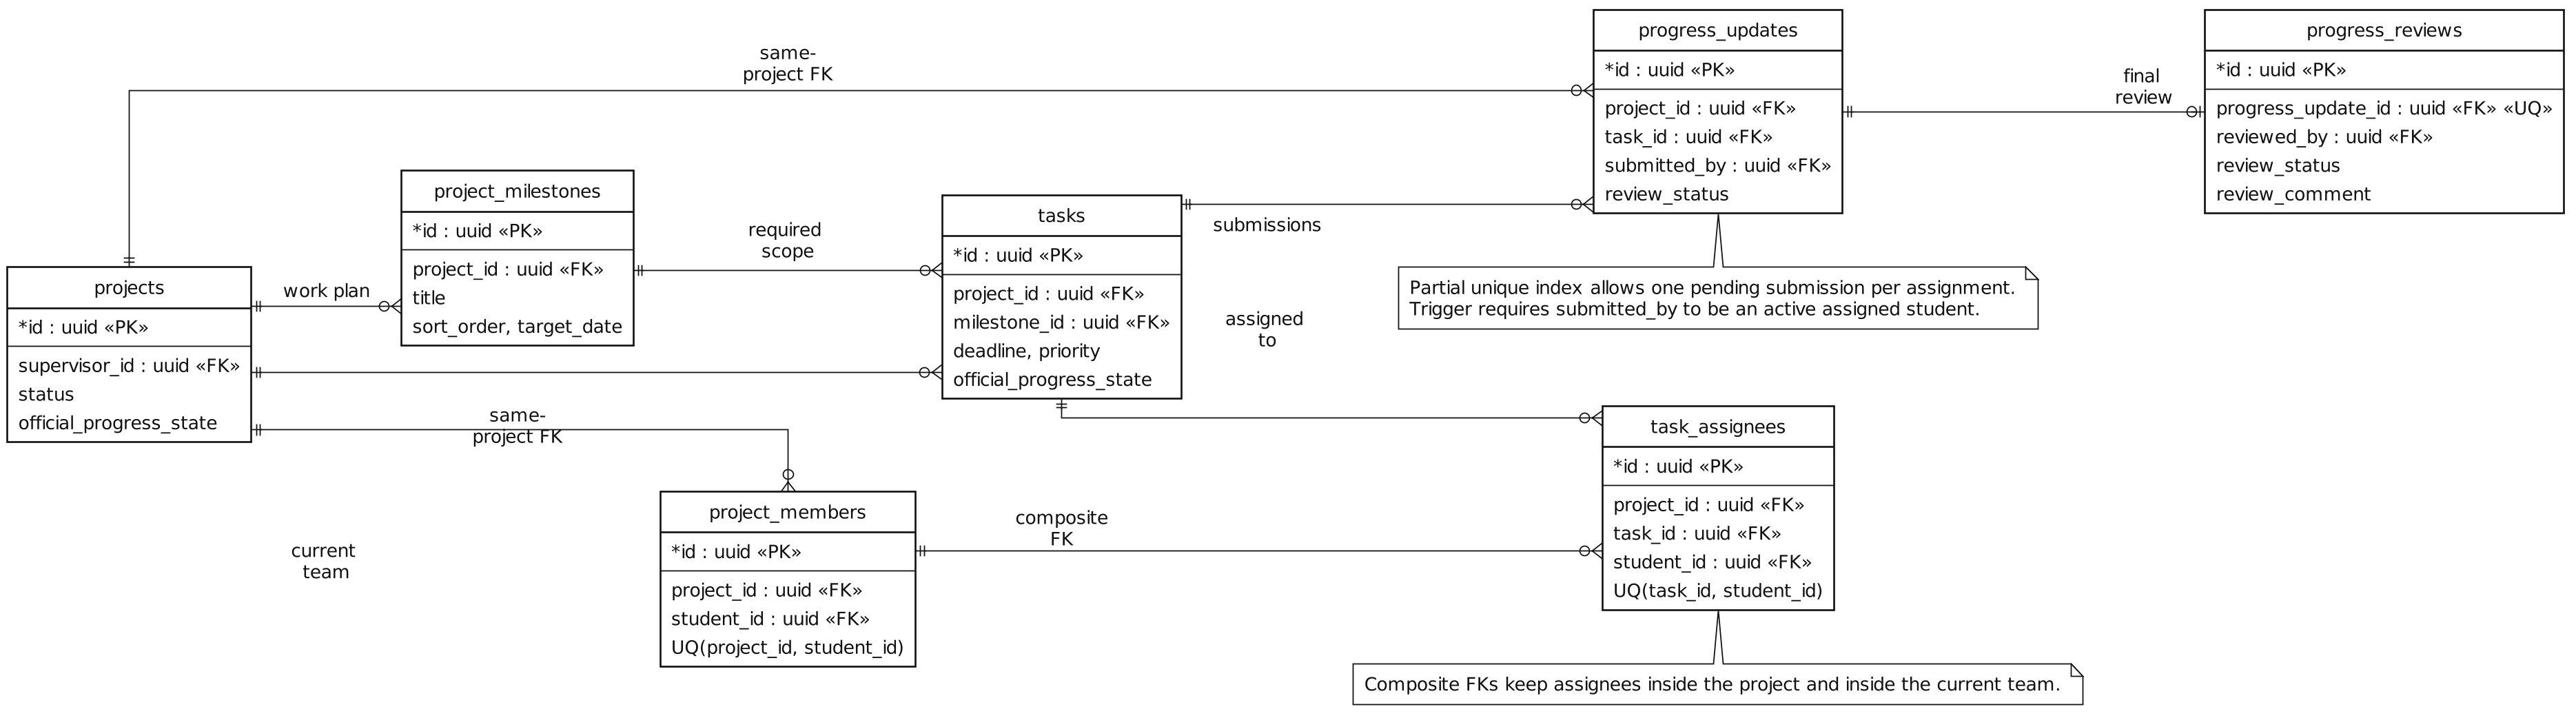
\includegraphics[width=\textwidth,height=0.45\textheight,keepaspectratio]{data-model-assignment.png}
  \vspace{0.25cm}
  \begin{columns}[T,totalwidth=\textwidth]
    \begin{column}{0.48\textwidth}
      \redtag{Trục dữ liệu}
      \begin{tightitems}
        \item \texttt{projects} là trung tâm.
        \item \texttt{milestones -> tasks -> submissions -> reviews}.
        \item Tài nguyên/file gắn theo đúng target nghiệp vụ.
      \end{tightitems}
    \end{column}
    \begin{column}{0.48\textwidth}
      \redtag{Invariant chính}
      \begin{tightitems}
        \item Người được giao phải thuộc cùng dự án.
        \item Một pending submission cho mỗi nhiệm vụ.
        \item Minh chứng đã duyệt không được sửa/xóa.
      \end{tightitems}
    \end{column}
  \end{columns}
\end{frame}

% 9
\settemplatebg{image12.png}
\begin{frame}{Bảo mật và kiểm soát request}
  \begin{columns}[T,totalwidth=\textwidth]
    \begin{column}{0.52\textwidth}
      \begin{tightitems}
        \item Session cookie HttpOnly; backend chỉ lưu token hash.
        \item Origin guard chặn request ghi từ nguồn không tin cậy.
        \item Strict JSON: giới hạn body, từ chối field lạ và JSON nối tiếp.
        \item Ghi dữ liệu theo dự án phải khóa transaction và đọc lại trạng thái mới nhất.
        \item PostgreSQL chặn dữ liệu sai bằng FK, unique index, trigger.
      \end{tightitems}
    \end{column}
    \begin{column}{0.43\textwidth}
      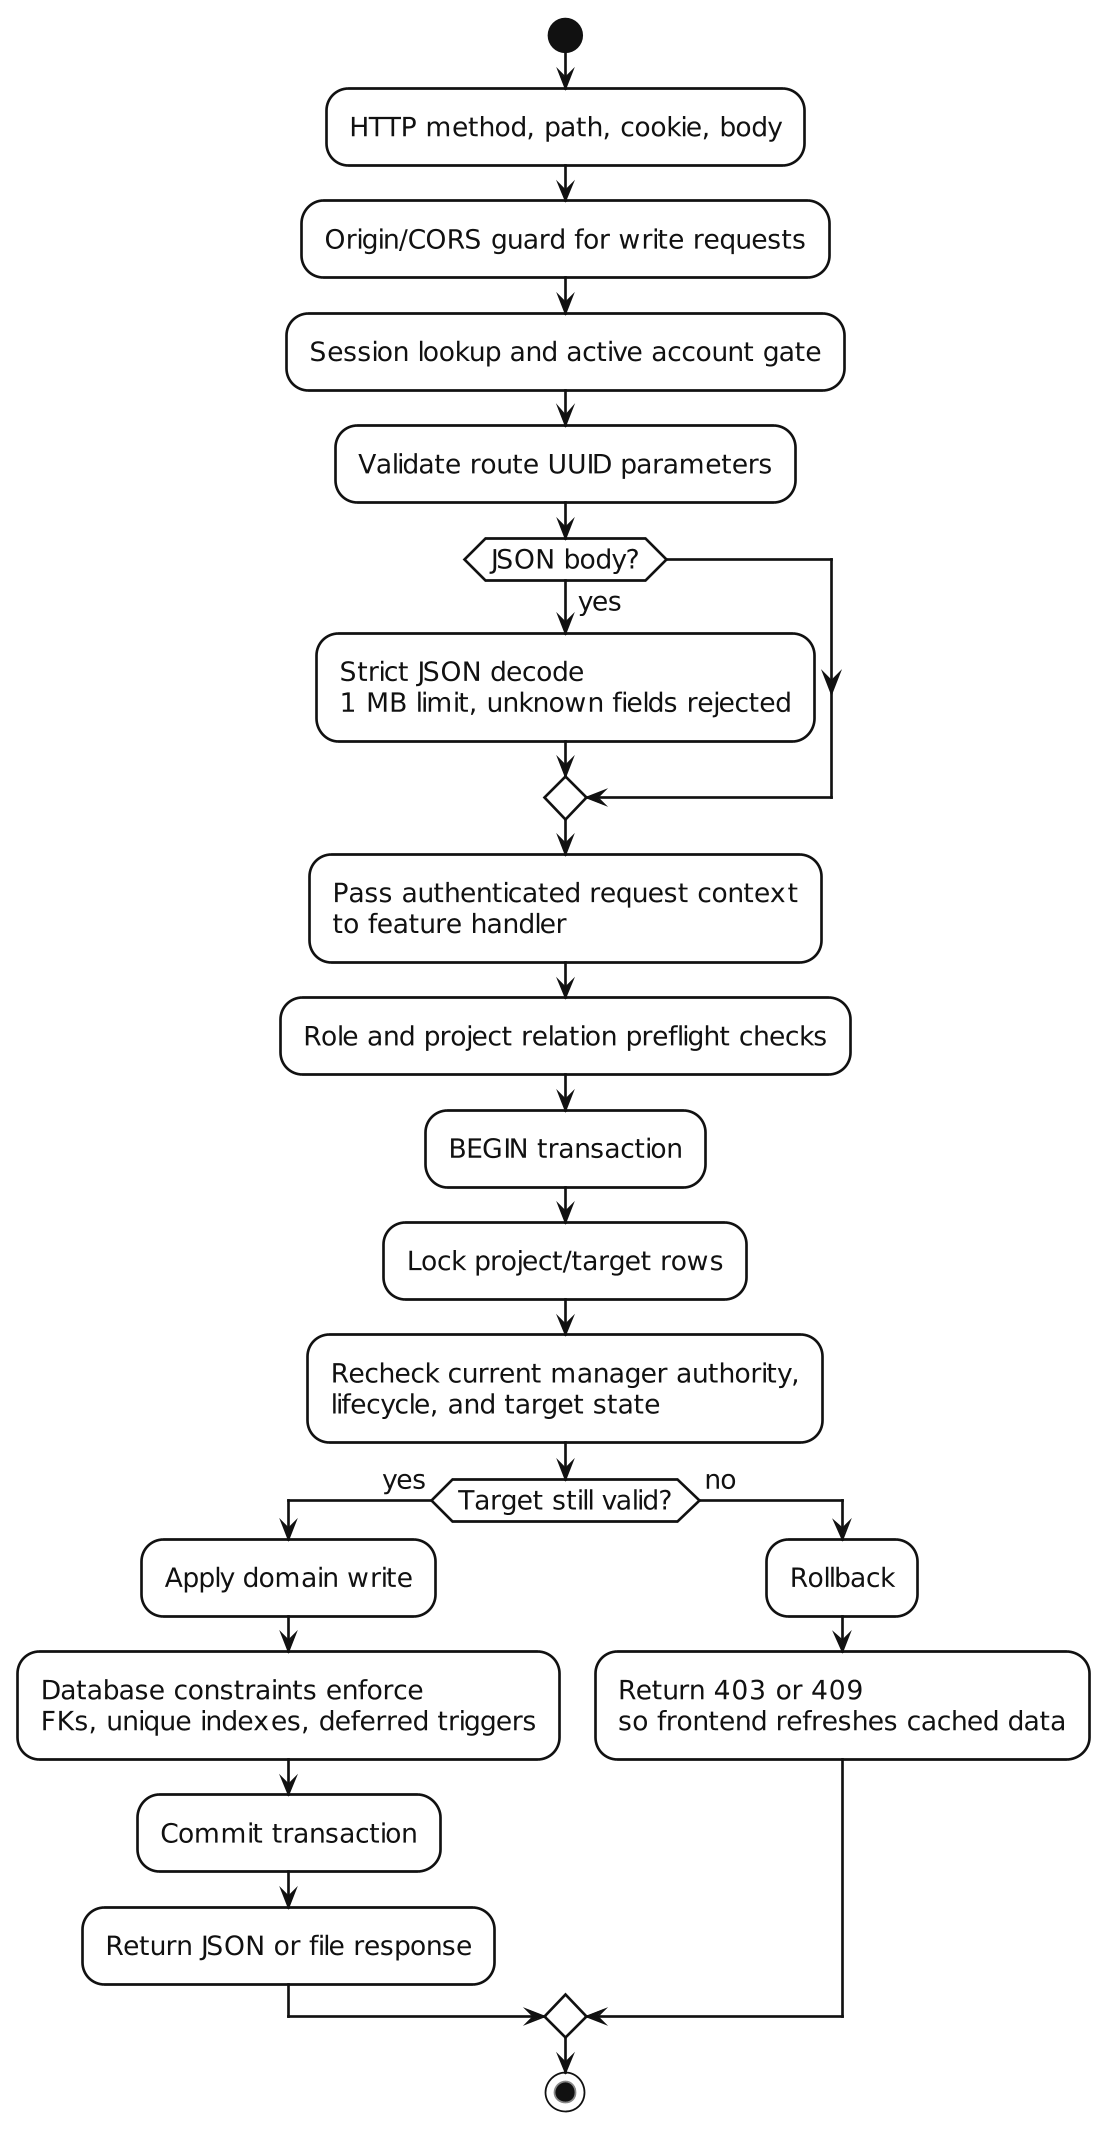
\includegraphics[width=\linewidth,height=0.72\textheight,keepaspectratio]{request-boundary.png}
    \end{column}
  \end{columns}
\end{frame}

% 10
\settemplatebg{image5.png}
\begin{frame}{Giao diện chính}
  \begin{columns}[T,totalwidth=\textwidth]
    \begin{column}{0.49\textwidth}
      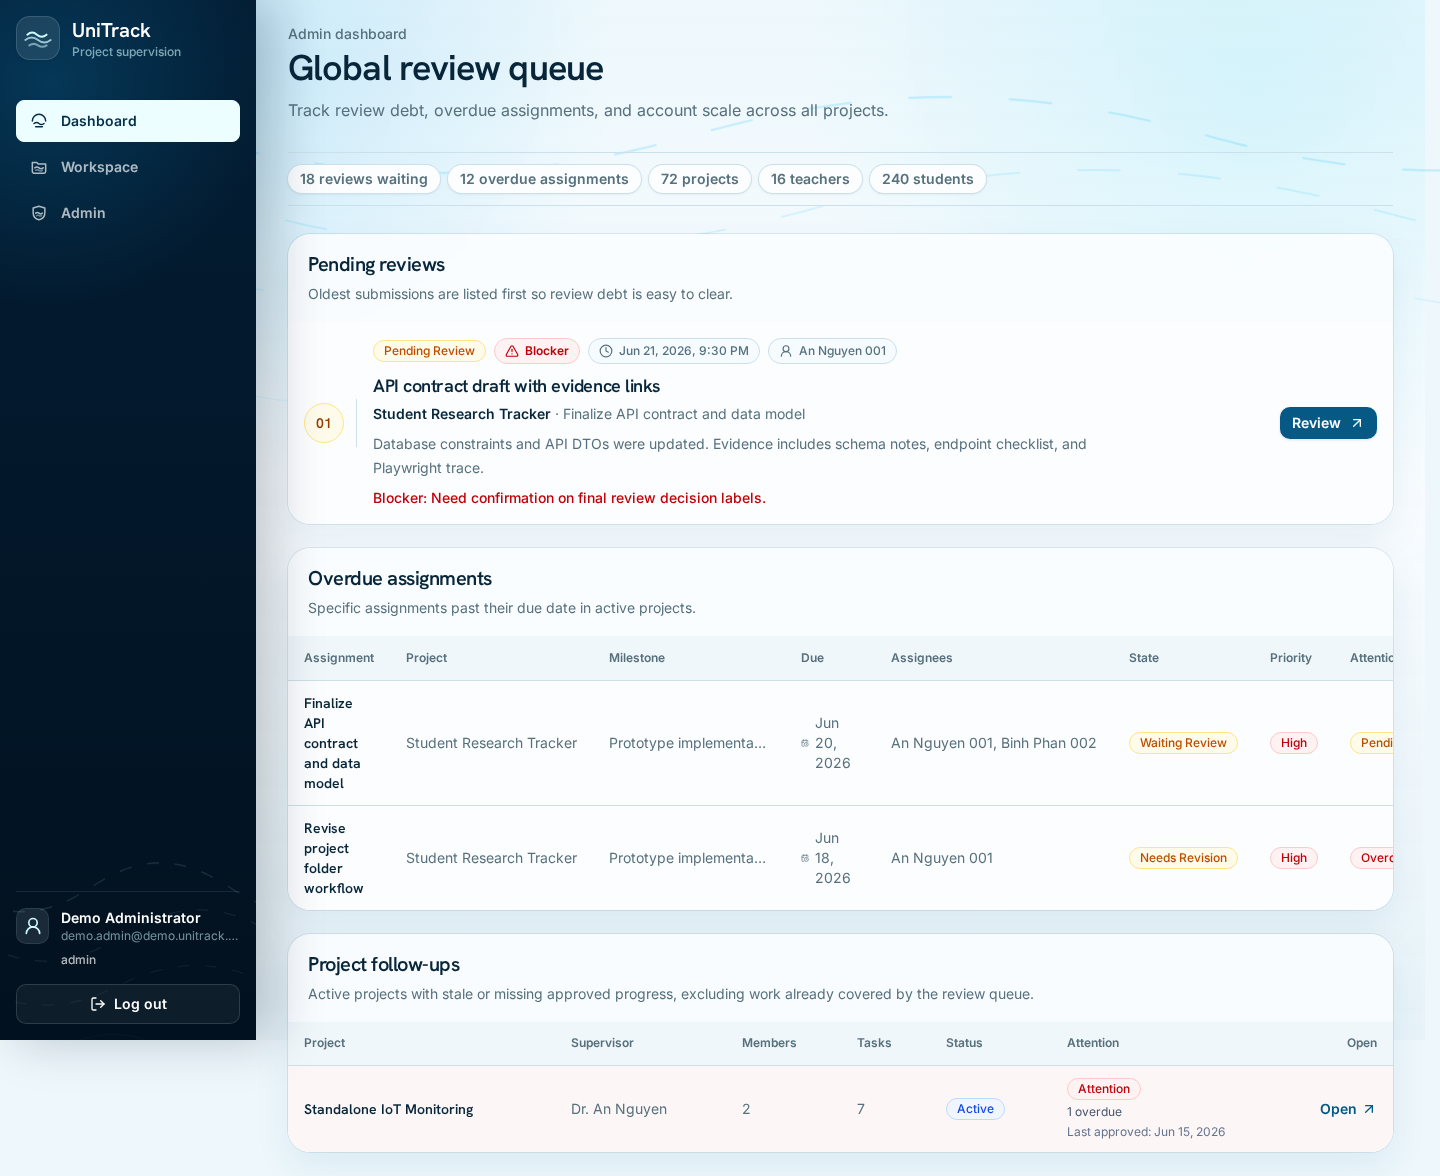
\includegraphics[width=\linewidth,height=0.36\textheight,keepaspectratio]{dashboard-admin.png}
      \vspace{0.1cm}
      {\scriptsize\textbf{Dashboard}: hàng đợi theo vai trò, bài chờ duyệt, nhiệm vụ quá hạn.}
    \end{column}
    \begin{column}{0.49\textwidth}
      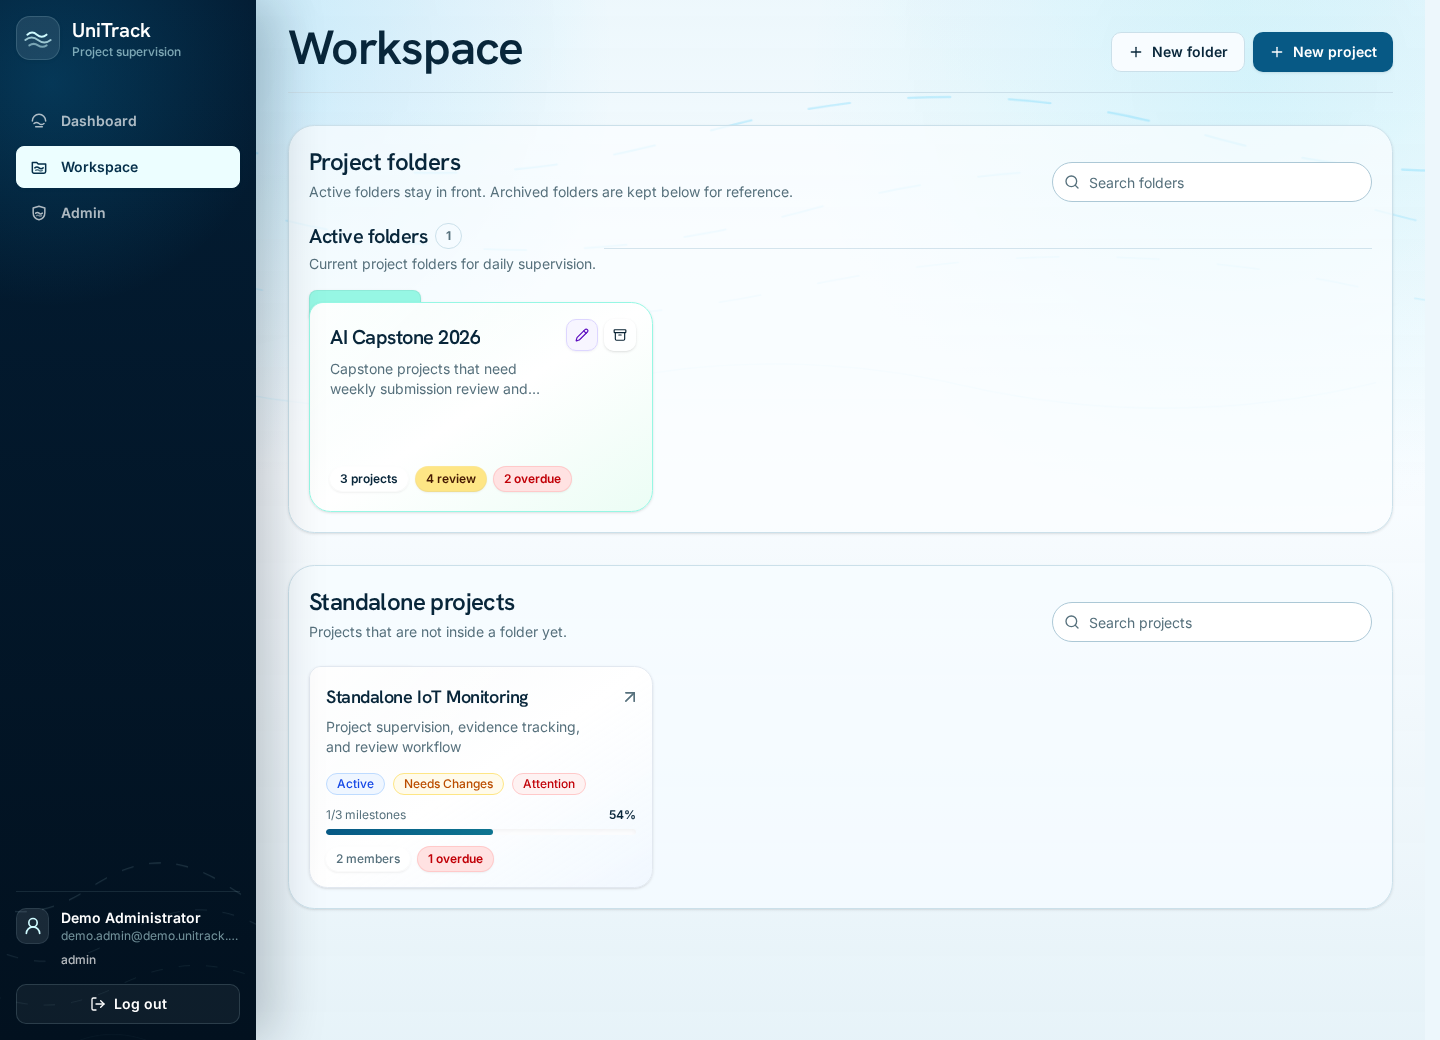
\includegraphics[width=\linewidth,height=0.36\textheight,keepaspectratio]{workspace.png}
      \vspace{0.1cm}
      {\scriptsize\textbf{Workspace}: thư mục dự án và danh sách dự án độc lập.}
    \end{column}
  \end{columns}
  \vspace{0.28cm}
  \begin{columns}[T,totalwidth=\textwidth]
    \begin{column}{0.49\textwidth}
      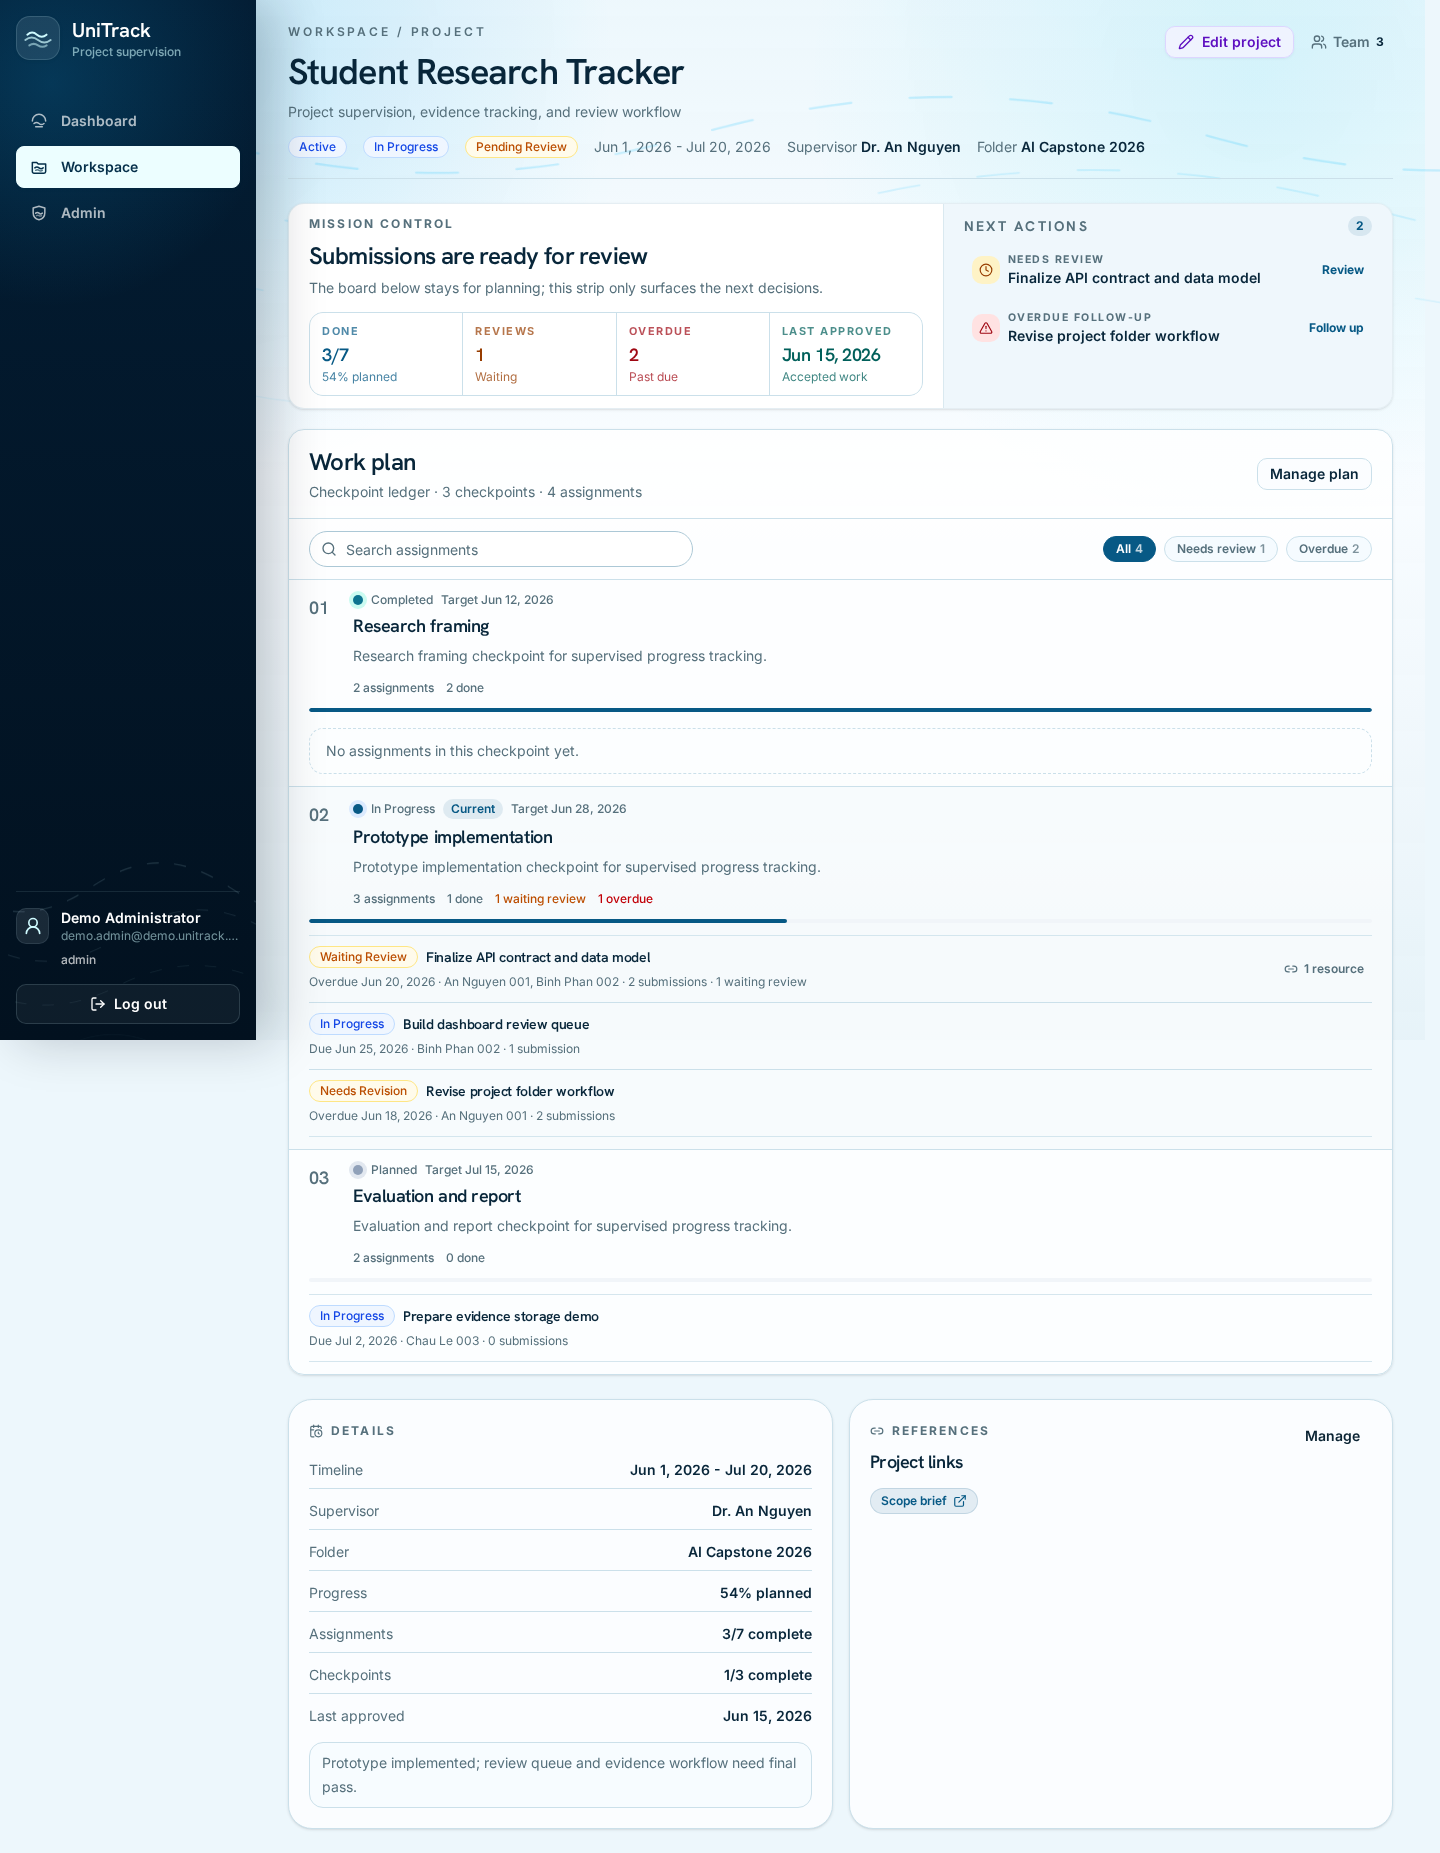
\includegraphics[width=\linewidth,height=0.25\textheight,keepaspectratio]{project-detail.png}
      {\scriptsize\textbf{Dự án}: hồ sơ, nhóm, kế hoạch công việc.}
    \end{column}
    \begin{column}{0.49\textwidth}
      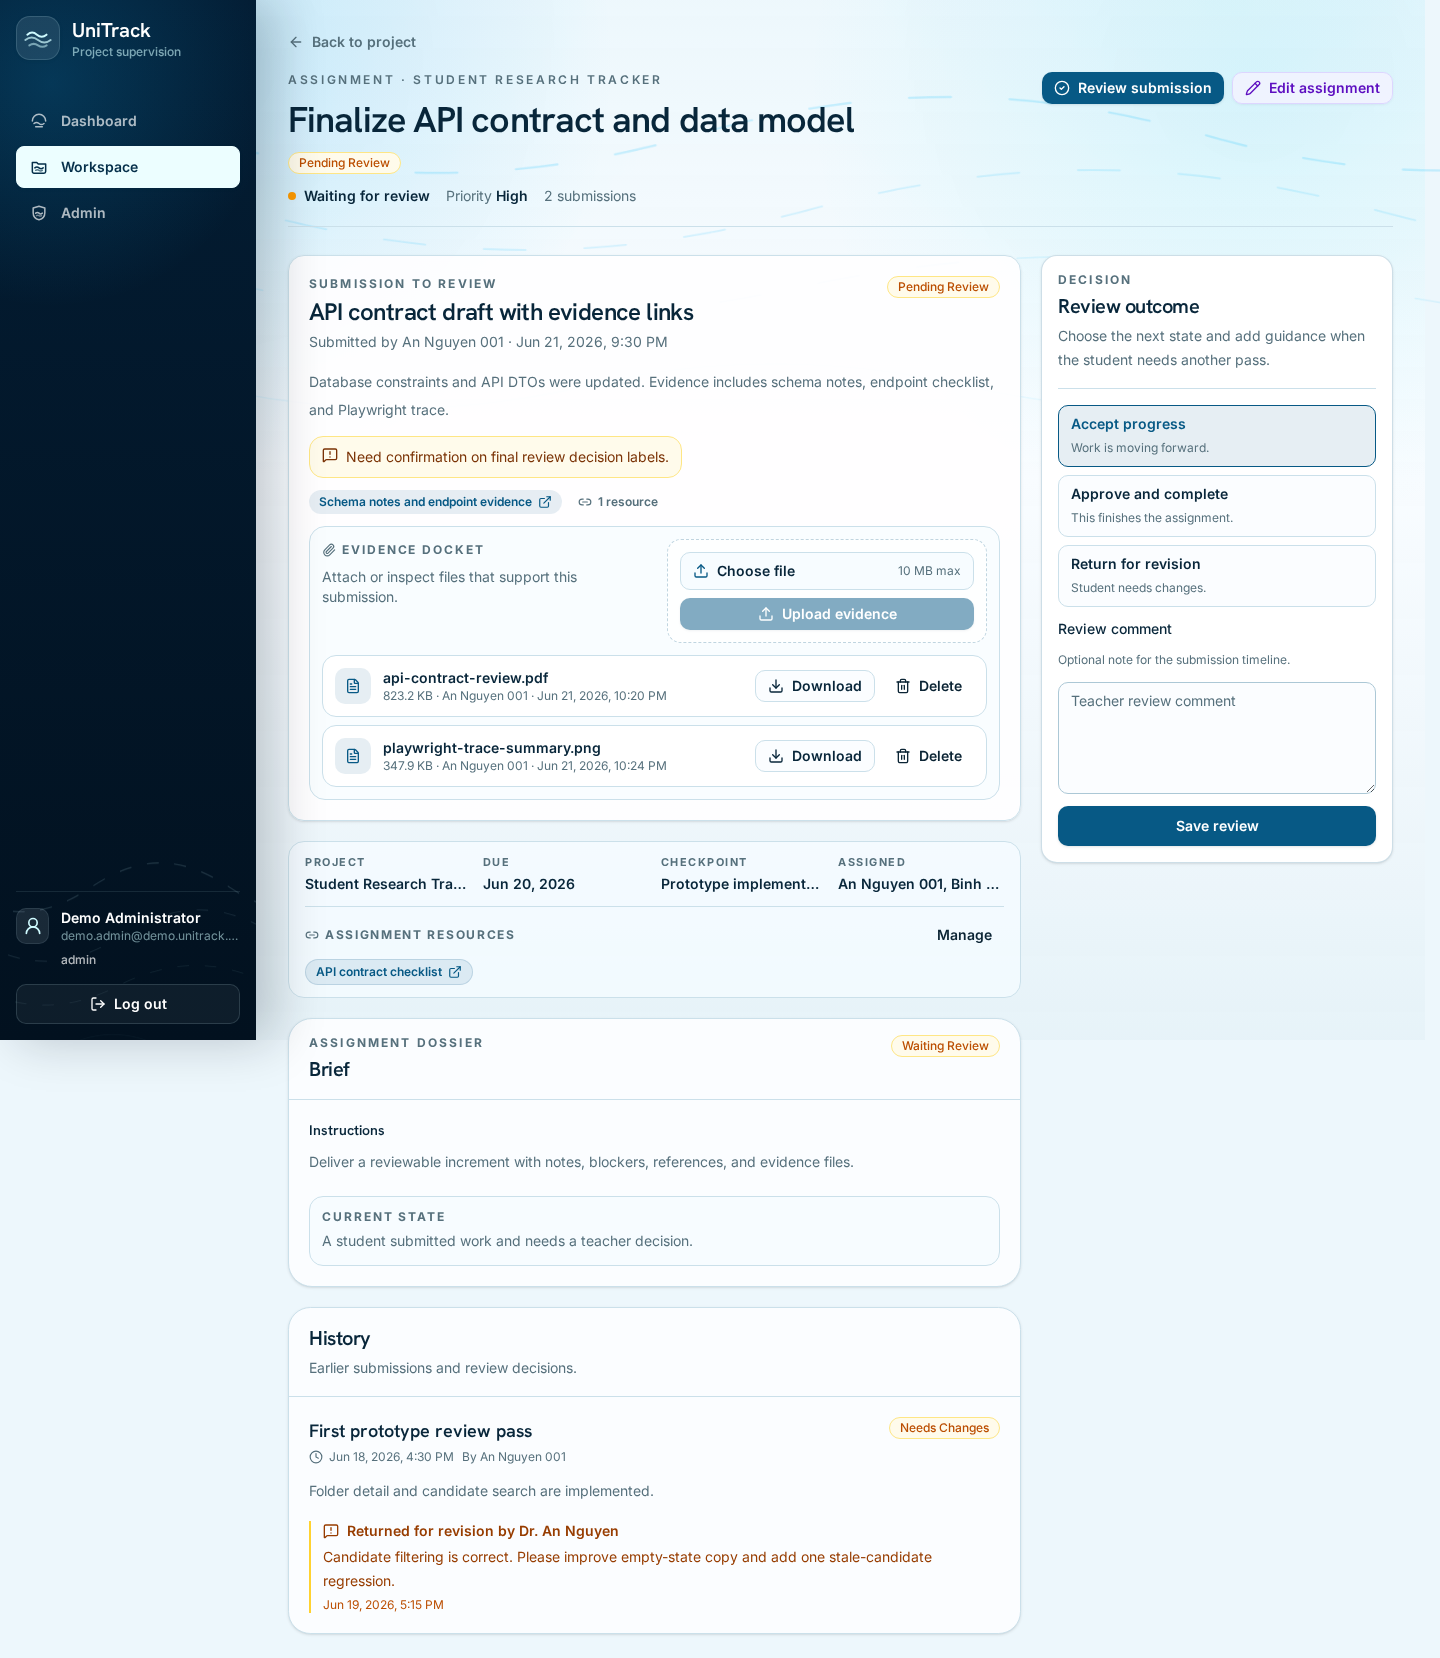
\includegraphics[width=\linewidth,height=0.25\textheight,keepaspectratio]{assignment-review-desk.png}
      {\scriptsize\textbf{Duyệt bài}: ngữ cảnh, minh chứng, quyết định.}
    \end{column}
  \end{columns}
\end{frame}

% 11
\settemplatebg{image6.png}
\begin{frame}{Luồng nộp bài và duyệt bài}
  \begin{columns}[T,totalwidth=\textwidth]
    \begin{column}{0.53\textwidth}
      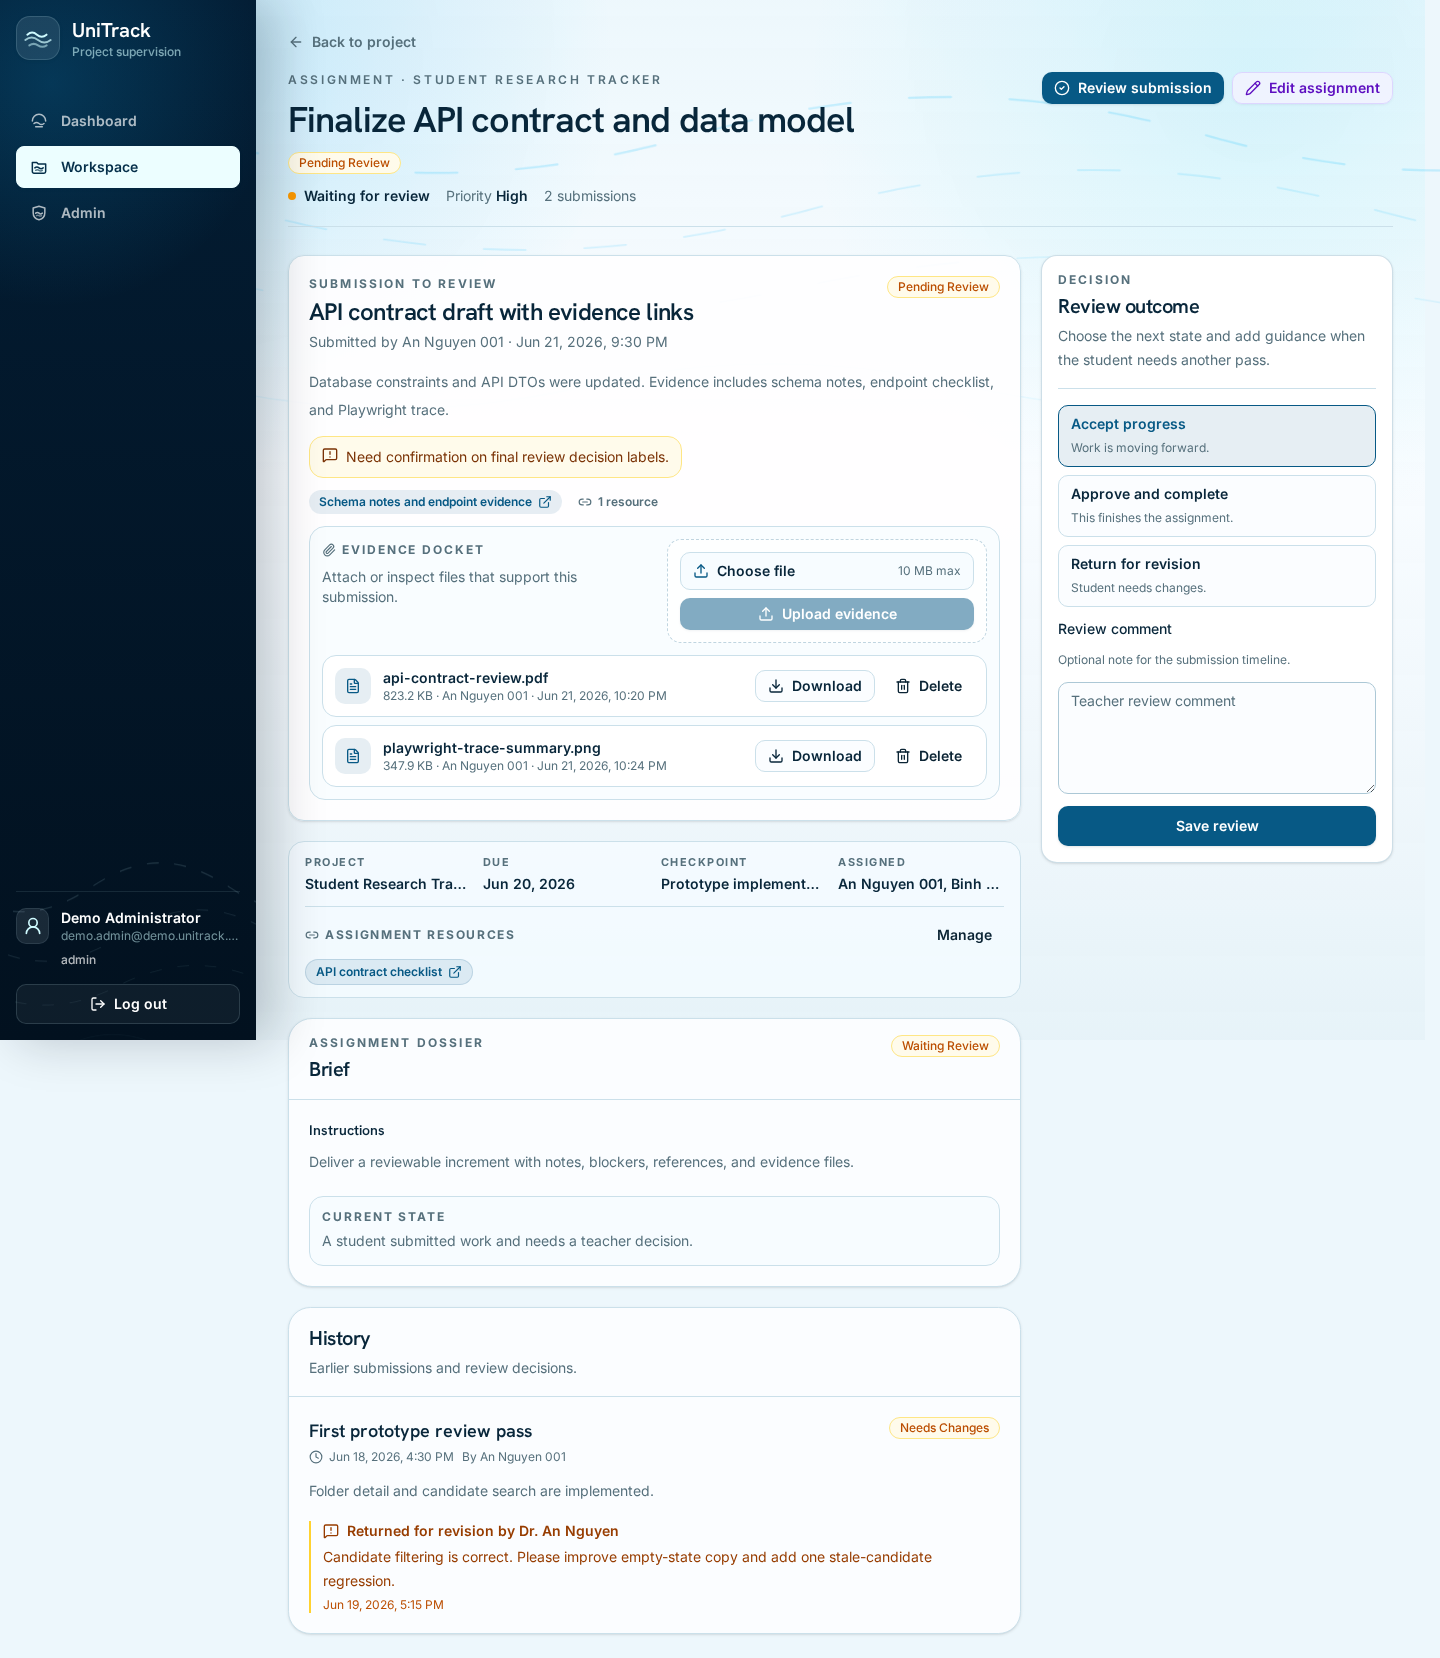
\includegraphics[width=\linewidth,height=0.68\textheight,keepaspectratio]{assignment-review-desk.png}
    \end{column}
    \begin{column}{0.43\textwidth}
      \redtag{Điểm chính}
      \begin{tightitems}
        \item Sinh viên nộp tiến độ theo nhiệm vụ được giao.
        \item Link tài nguyên và file minh chứng gắn với bài pending.
        \item Giảng viên duyệt một lần: accepted, revision, rejected.
        \item Sau duyệt, tài nguyên và file chuyển sang chỉ đọc.
      \end{tightitems}
      \vspace{0.2cm}
      \colorbox{hustlight}{\parbox{0.95\linewidth}{\small Mục tiêu: quyết định đánh giá có ngữ cảnh và minh chứng tin cậy.}}
    \end{column}
  \end{columns}
\end{frame}

% 12
\settemplatebg{image7.png}
\begin{frame}{Dấu vết triển khai trong codebase}
  \small
  \renewcommand{\arraystretch}{1.22}
  \begin{tabularx}{\textwidth}{>{\bfseries\color{hustred}}p{2.7cm}X}
    Auth/account & \smallpath{apps/api/internal/app/auth.go}, \smallpath{admin\_users.go}, \smallpath{apps/web/src/features/auth} \\
    Project/task & \smallpath{apps/api/internal/app/projects.go}, \smallpath{tasks.go}, \smallpath{milestones.go} \\
    Frontend UI & \smallpath{apps/web/src/features/dashboard}, \smallpath{workspace}, \smallpath{projects}, \smallpath{tasks} \\
    Data integrity & \smallpath{apps/api/db/migrations/20260619...}, \smallpath{20260620...}, \smallpath{20260621...} \\
    Resources/files & \smallpath{apps/api/internal/app/resources.go}, \smallpath{files.go}, \smallpath{storage.go} \\
    Testing & \smallpath{apps/api/internal/app/*\_test.go}, \smallpath{apps/web/e2e/*.spec.ts}
  \end{tabularx}

  \vspace{0.35cm}
  \begin{block}{Cách tổ chức}
    \small Codebase giữ theo lát tính năng: UI, API, state/query, migration và test bám cùng workflow nghiệp vụ.
  \end{block}
\end{frame}

% 13
\settemplatebg{image8.png}
\begin{frame}{Kiểm thử và đánh giá}
  \begin{columns}[T,totalwidth=\textwidth]
    \begin{column}{0.48\textwidth}
      \redtag{Kiểm thử}
      \begin{tightitems}
        \item Backend: session, permission, lifecycle lock, storage, trigger.
        \item Validation: JSON sai, route ID sai, stale request, file quá lớn.
        \item Playwright: login, admin, dashboard, access-control, accessibility.
      \end{tightitems}
    \end{column}
    \begin{column}{0.48\textwidth}
      \redtag{Kết quả}
      \begin{tightitems}
        \item Workflow lõi đã hoạt động end-to-end.
        \item Phân quyền và vòng đời dự án được kiểm soát ở backend.
        \item Database bảo vệ quan hệ cùng dự án và minh chứng sau duyệt.
      \end{tightitems}
    \end{column}
  \end{columns}
  \vspace{0.35cm}
  \colorbox{hustlight}{\parbox{0.94\textwidth}{\small Hạn chế: chưa có audit UI, quản lý toàn bộ dự án cho admin, hardening storage production và độ phủ Playwright rộng hơn.}}
\end{frame}

% 14
\settemplatebg{image11.png}
\begin{frame}{Kết luận và hướng phát triển}
  \begin{columns}[T,totalwidth=\textwidth]
    \begin{column}{0.48\textwidth}
      \redtag{Kết luận}
      \begin{tightitems}
        \item UniTrack đáp ứng luồng project-first cho đồ án sinh viên.
        \item Điểm nổi bật là phối hợp UI, backend và database để bảo vệ dữ liệu.
        \item Hệ thống có nền tảng tốt để tiếp tục mở rộng theo từng lát nhỏ.
      \end{tightitems}
    \end{column}
    \begin{column}{0.48\textwidth}
      \redtag{Hướng phát triển}
      \begin{tightitems}
        \item Quản lý toàn bộ dự án và audit log cho admin.
        \item Thông báo trong hệ thống/email.
        \item Quota, MIME allowlist, quét mã độc, backup cho minh chứng.
        \item Mở rộng Playwright cho form và file/resource flow.
      \end{tightitems}
    \end{column}
  \end{columns}
\end{frame}

% 15
\settemplatebg{image9.png}
\begin{frame}[plain]
  \vspace{2.05cm}
  \centering
  {\fontsize{28}{32}\selectfont\bfseries\color{hustred} Xin cảm ơn!}\par
  \vspace{0.45cm}
  {\Large\bfseries Q \& A}\par
  \vspace{0.65cm}
  {\small \StudentName}\par
  {\small \StudentEmail}
\end{frame}

\end{document}
